\chapter{\label{chap:grundlagen}Grundlagen}
Dieses Kapitel befasst sich mit sowohl den mathematischen als auch den technischen Grundlagen der zu behandelnden Thematik, welche für das weitere Verständnis der Arbeit beitragen.
% -------------------------------------------------
% TECHNISCHE GRUNDLAGEN
% -------------------------------------------------
\section{\label{sec:technGrundlagen}Technische Grundlagen}
Erstellt wird eine Smartphone Anwendung, deren Grundlage für die Implementierung die Software-Plattform Android ist. Im folgenden Abschnitt werden Funktionsweise und Besonderheiten der verwendeten Technologien beschrieben. 
% ANDROID
\subsection{Android}
Die umfassende Open-Source-Plattform Android stellt eine vollständige Ausstattung für Mobilgeräte dar. Android-Anwendungen werden mit der Programmiersprache Java und der Auszeichnungssprache \gls{XML} entwickelt. Mit dem Android \gls{SDK}\footnote{ Das Android \gls{SDK} steht unter \url{https://developer.android.com/sdk/index.html} zum Download bereit} werden die Werkzeuge und \gls{API} zur Verfügung gestellt, die erforderlich sind Mobilanwendungen auf der Android-Plattform erzeugen zu können.\\ 
Zu den wichtigsten \gls{SDK} Werkzeugen gehören der Android \gls{SDK}-Manager\footnote{ Der \gls{SDK}-Manager verwaltet die \gls{SDK}-Pakete, sowie die installierten Pakete imd System-Images}, der AVD-Manager\footnote{ Der AVD-Manager bietet eine grafische Oberfläche in der Android Virtuell Devices verwaltet und im Emulator ausgeführt werden können.}, der Emulator und der Dalvik Debug Monitor Server\footnote{ Mithilfe des Ddms können Android Anwendungen auf Fehler untersucht werden} (Ddms). Die Virtuelle Maschine Dalvik wurde unter Berücksichtigung von Rechenleistung und der Lebensdauer von Batterien speziell von Google für Android entworfen. \cite{android_sdk} Ab Android 4.4 wird die Android Runtime (ART) als alternative zur Dalvik \gls{VM} angeboten. Diese bietet eine Reihe von neuen Funktionen die die Laufzeit verbessern. \cite{android:art}\\
Mit dem Android \gls{NDK}\footnote{ Das Android \gls{NDK} steht unter \url{https://developer.android.com/tools/sdk/ndk/index.html} zum Download bereit} existiert auch ein Tool, mit dem Teile einer Anwendung in systemeigenen Programmiersprachen wie C oder C++ implementiert werden können. Programmcode, der in solchen Sprachen eignet, ist zum Beispiel bei CPU-intensiven Operationen wie Signalverarbeitungen oder Physik-Simulationen. Hier ist sicherzustellen, ob die erforderlichen Bibliotheken in dem \gls{SDK} auch verfügbar sind. \cite{android_ndk} \\
Einen Überblick über die komplexe Android-Systemarchitektur, welche nachfolgend (nach \cite{android} S. 3ff) kurz beschrieben wird, zeigt die folgende Abbildung \ref{fig:android}.
\begin{figure}[H]  
    \centering  
    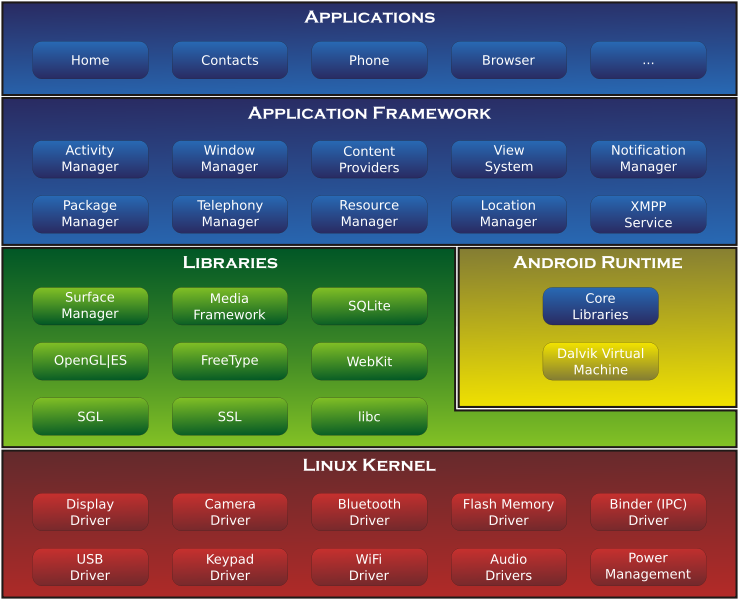
\includegraphics[width=0.7\textwidth]{Android-System-Architecture} 
    \caption[Android-Systemarchitektur]{Die Android-Systemarchitektur Quelle: \url{http://en.wikipedia.org/wiki/File:Android-System-Architecture.svg}}
    \label{fig:android}
\end{figure}
\paragraph{Linux Kernel: }
Android basiert auf dem Linux 3.1-Kernel. Dieser eine bewährte Betriebssystemgrundlage indem er die erforderlichen Hardware-Treiber zur Verfügung stellt.
\paragraph{Bibliotheken: }
Systemeigenen Bibliotheken sind C/C++ Bibliotheken und vorinstalliert. Dazu gehören alle Bibliotheken im grünen Bereich von Abbildung \ref{fig:android}:
\begin{itemize}[leftmargin=0.7cm]
\renewcommand\labelitemi{--}
	\item \textsc{Surface Manager} ~ Der für das individuelle Display Verwaltung verantwortliche Oberflächen-Manager
	\item \textsc{OpenGL/ES} ~ Eine 2D und 3D Grafikbibliothek
	\item \textsc{SGL} ~ Eine 2D Grafikbibliothek
 	\item \textsc{Media-Framework} ~ eine Medien-Bibliothek zur Wiedergabe von Audio- und Video-Daten 	
 	\item \textsc{FreeType} ~ eine Bibliothek zur Darstellung von Computerschriften als Rastergrafik
 	\item \textsc{SSL} ~ Das Secure-Socket-Layer für die Internet-Sicherheit
	\item \textsc{SQLite} ~ Ist eine ausgereifte Datenbank die den internen Speicher nutzt 
	\item \textsc{Webkit} ~ WebKit ist die Standard-Browser-Engine und erlaubt das schnelle Rendern und Anzeigen von HTML Seiten
	\item \textsc{libc} ~ C-Bibliothek
\end{itemize}
\paragraph{Android Runtime: }
Die Android Laufzeitumgebung nutzt die Java-Core-Bibliotheken und die Dalvik \gls{VM}. 
Die Dalvik \gls{VM} ist Googles Implementation von Java, zur Anwendung auf mobilen Geräten optimiert. Jede gestartete Android-Anwendung läuft in einem eigene Prozess und bekommt darüber hinaus seine eigene Dalvik \gls{VM}. Da die Anwendungen über keinen gemeinsamen Speicher verfügen erhöht das die Sicherheit und Verfügbarkeit und ist somit optimaler, obwohl mehr Ressourcen benötigt werden. Denn ein sterbender Prozess nimmt so nur seine "'eigene"' Anwendung mit. \\ 
Die Anwendungen werden zunächst von einem normalen Java-Compiler in Java-Bytecode übersetzt und dann von dem Dex-Compiler in den Dalvik-Bytecode, welcher schließlich von der Dalvik \gls{VM} ausgeführt wird.
\paragraph{Application Framework: }
Androids Application-Framework ist eine Umgebung die unterschiedliche DIenste zur Verfügung stellt. Sie bietet EntwicklerInnen Zugriff auf die im Kern verwendeten \glspl{API} sowie auf die Java-Bibliotheken die für Android erstellt wurden. 
\paragraph{Applications: }
Auf der obersten Ebene in Abbildung \ref{fig:android} befinden sich die Anwendungen die den täglichen Telefon-Bedarfs wie Adressbuch, Messenger, E-Mail, Internet-Browser etc. decken. Zusätzlich unterstützt Android verschiedene Anwendungen von Drittanbietern. Diese sind hauptsächlich in Java geschrieben und werden am häufigsten über den Google Play Store verteilt.
\subsection{Die native Datenbank SQLite}
% MOBILE SENSING
\subsection{Mobile Sensorik} 
\subsubsection{Mobile Sensorik unter Android}
\subsubsection{Geolokation mittels \gls{GPS}}
\subsubsection{G-Sensor}
Blabla Beschleunigungssensor...
\clearpage
% -------------------------------------------------
% MATHEMATISCHE GRUNDLAGEN
% -------------------------------------------------
\section{\label{sec:mathGrundlagen}Berechnung der Geschwindigkeitsempfehlung}
Präsentiert das System während der Anwendung eine Geschwindigkeitsempfehlung, ist diese abhängig von der Fahrtgeschwindigkeit und vom Abstand zur Ampel. Angenommen die Progressionsgeschwindigkeit $v$ wird zum Zeitpunkt $t_{1}$ ermittelt, die \gls {LSA} schaltet zum Zeitpunt $t_{2}$ auf Rot und Abstand zur Ampel beträgt $s$, dann gilt: \\
\[ v = \frac{s}{t_{2} - t_{1}} \] \\
Der Abstand zur Ampel wird also durch die verbleibende Zeit dividiert. 
Die von der Berliner Verkehrsleitzentrale zur Verfügung gestellten Ampelschaltpläne und Position der angesteuerten Ampel dienen als Grundlage dieser Berechnung und sind aus der Datenbank zu holen. Die aktuelle Position des Fahrrads wird vom \gls{GPS} Sensor des \glspl{Smartphone} ermittelt und daraus der Abstand zur Ampel errechnet. Die Abbildung \ref{fig:vst} soll die Berechnungsgrundlagen veranschaulichen: 
\begin{figure}[H]  
    \centering  
    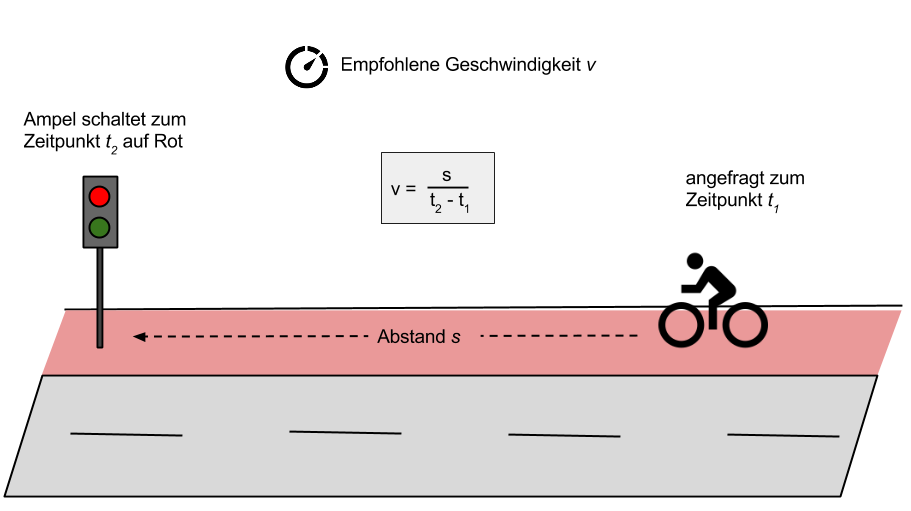
\includegraphics[width=1\textwidth]{vst}     
    \caption[Berechnung Progressionsgeschwindigkeit]{Veranschaulichung der Berechnung}
    \label{fig:vst}
\end{figure}
Um die ensprechende \gls{LSA} während der Grünphase zu passieren, muss letztendlich die empfohlene Geschwindigkeit $v$ eingehalten werden.
